\section{Wohlstand}
\subsection{Preismechanismus und Marktwirtschaft \ho{Ho2}}
\subsubsection{Ausgangslage \ho{Ho2 F4}}
Unbeschr�nkte Bed�rfnisse vs. knappe Ressourcen.
\subsubsection{Opportunit�tskosten \ho{Ho2 F4-6}}
  Kosten, die bei einer Entscheidung anfallen, dass die Vorteile einer
  Handlungsalternative nicht realisiert werden k�nnen.\\
  Beispiel: Weil wir studieren verdienen wir derzeit nichts/weniger. Das Geld
  das wir dadurch verlieren sind die Opportunit�tskosten.\\
  Die Opportunit�tskosten zeigen die Knappheit eines Gutes an.
\subsubsection{Zentrale Rolle der Preise in der Marktwirtschaft \ho{Ho2 F8-9}}
  Der Preis wird von der Nachfrage bestimmt und hat Signalwirkung. Steigt er so
  ist das ein anzeichen f�r knappheit. Planwirtschaft zerst�rt das alles.
\begin{multicols}{2}
	\subsubsection{Mikro�konomisches Grundmodell \ho{Ho2 F10-12}}
	  \begin{tabular}{ll}
	    G�termarkt & Preis - Menge\\
	    Arbeitsmarkt & Lohn - Arbeit\\
	    Kapitalmarkt & Zins - Kapital\\
	  \end{tabular}
	  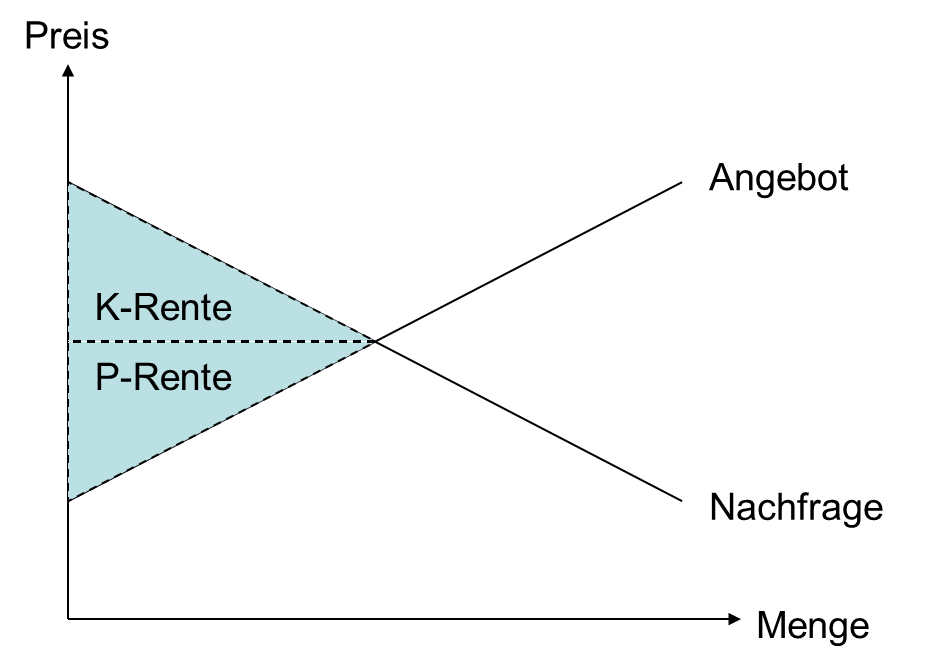
\includegraphics[width=8cm]{./bilder/h02f15.png}
	\subsubsection{Mindestpreis \ho{Ho2 F16-19}}
	  Auswirkungen wenn man einen Mindestpreis einf�hrt:\\
	  Konsum sinkt $\Rightarrow$ Angebot steigt $\Rightarrow$ Ware wird exportiert
	  oder vergammelt $\Rightarrow$ Konsumentenrente sinkt $\Rightarrow$
	  Produzentenrente steigt $\Rightarrow$ Gesamtrente sinkt.\\
	  Bei H�chstpreisen geschieht das ganze analog. Man sollte also nicht mit
	  Mindest/H�chstpreisen in den Markt eingreifen (auch bei L�hnen!).
	  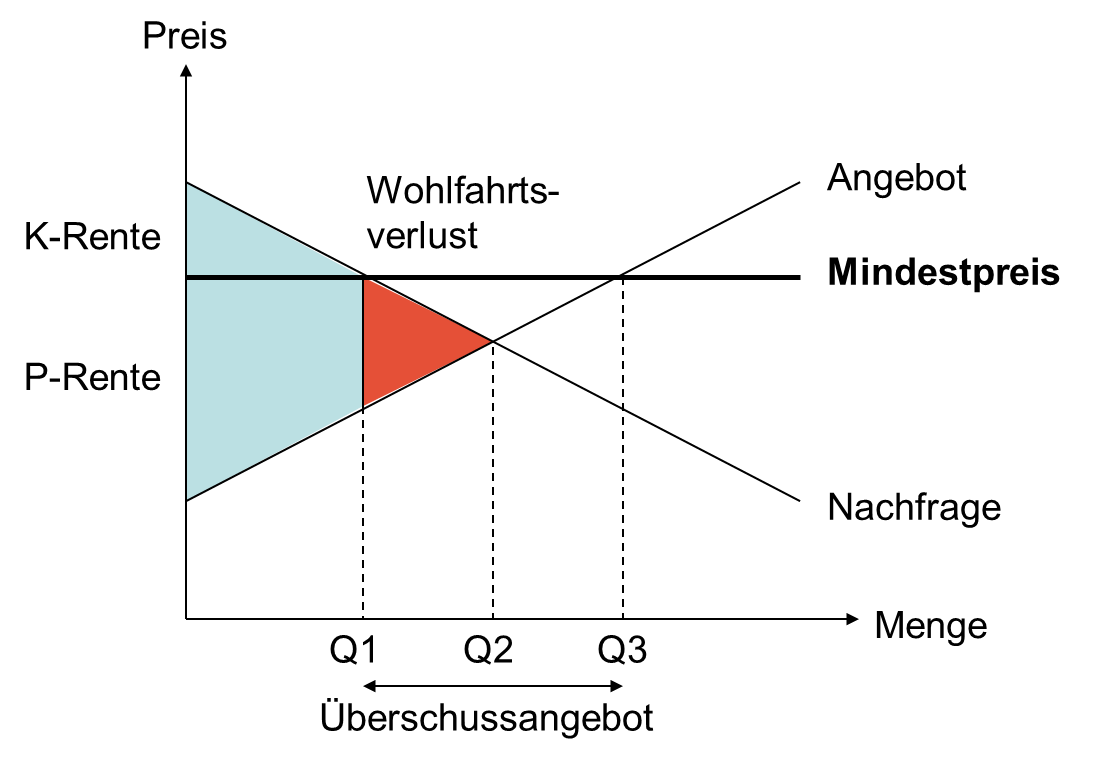
\includegraphics[width=8cm]{./bilder/h02f19.png}
\end{multicols}

\subsection{Internationale Arbeitsteilung \ho{Ho3}}
\subsubsection{Komparativer Kostenvorteil \ho{Ho3 F6}}
\begin{multicols}{2}
  Vorgehen:
  \begin{itemize}
    \item Opportunit�tskosten Berechnen f�r alle Artikel.
    \item Opportunit�tskosten vergleichen.
    \item Der Ort mit den tiefsten Opportunit�tskosten produziert und
    exportiert zu einem Preis zwischen Opportunit�tskosten im
    Exportort und den Opportunit�tskosten im Importort (nat�rlich nur ohne
    Z�lle, Transportkosten etc.).
  \end{itemize}
  Falls Gleichstand ist findet kein Handel statt.
  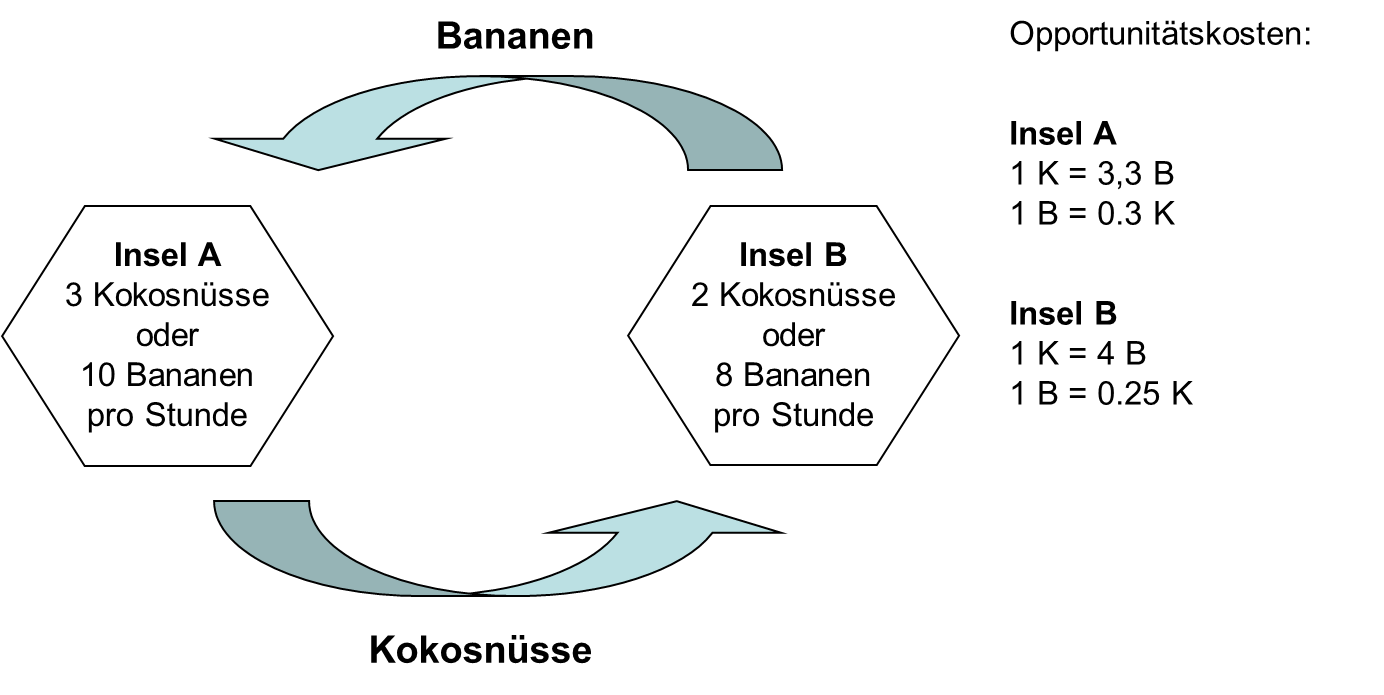
\includegraphics[width=9cm]{./bilder/h03f07.png}
\end{multicols}
\subsubsection{Weltmarktpreis \ho{Ho3 F8-13}}
Hoher Weltmarktpreis: Konsument verliert, Allgemeinheit und Produktion gewinnt.\\
Tiefer Weltmarktpreis bewirkt genau das Gegenteil.\\
Internationale Arbeitsteilung bringt positive Wohlfahrtseffekte unabh�ngig
davon, ob der Weltmarktpreis h�her oder tiefer als der Heimmarktpreis ist.
\begin{multicols}{2}
	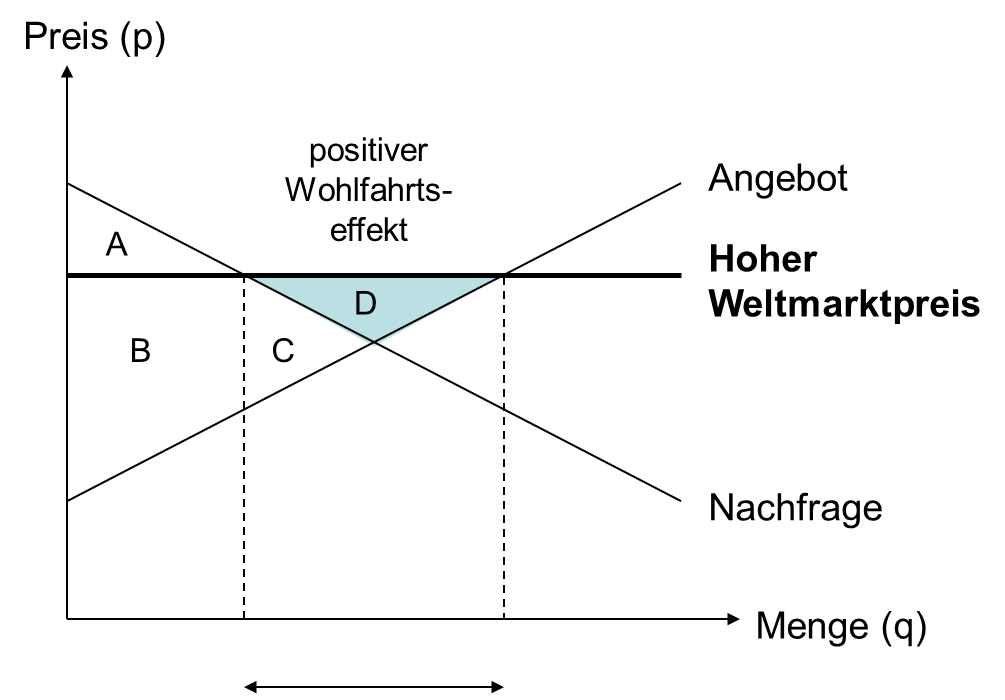
\includegraphics[width=9cm]{./bilder/h03f11.png}
	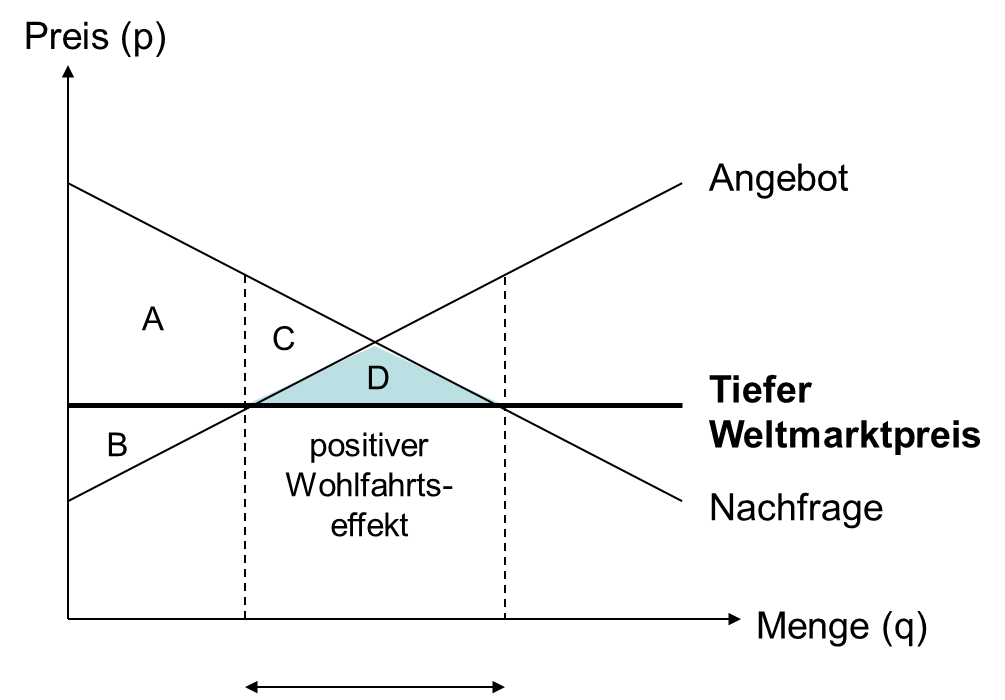
\includegraphics[width=9cm]{./bilder/h03f13.png}
\end{multicols}

\subsubsection{Z�lle \ho{Ho3 F15-17}}
\subsubsection{Regionale Integrationsr�ume \ho{Ho3 F22FF}}
\begin{multicols}{2}
\subsection{Monopolmacht und Wettbewerb \ho{Ho4}}
  Grenzkosten = Kosten f�r letztes produziertes Gut (zunehmend)\\
  Grenzertrag = Ertrag f�r letztes produziertes Gut (abnehmend)\\
  Bei einem Monopol sind die beiden gleich!
  
\subsubsection{Nat�rliche und nicht-nat�rliche Monopole \ho{Ho4 F19FF}}
  Ein typisches nat�rliches Monopol ist der Eisenbahnverkehr. Man kann nicht
  einer anderen Firma sagen sie soll ein zweites Gleis daneben bauen. Um das
  nat�rliche Monopol zu lockern kann man zum Beispiel die Schienen
  Verstaatlichen aber darauf Verkehr f�r mehrere Firmen zulassen (SBB, DB, SOB,
  BLS etc.). Anderes Beispiel: Strommarkt/netz
  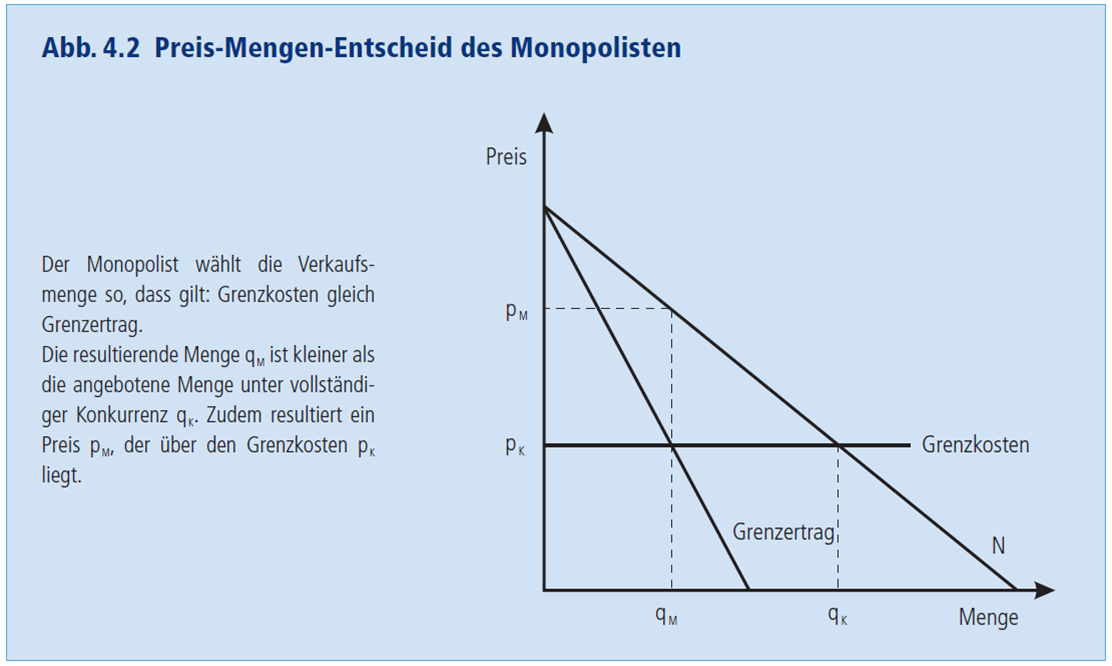
\includegraphics[width=9.5cm]{./bilder/h04f11.png}
\end{multicols}

\subsection{Externe Effekte und die Umwelt \ho{Ho5}}
\begin{multicols}{2}
	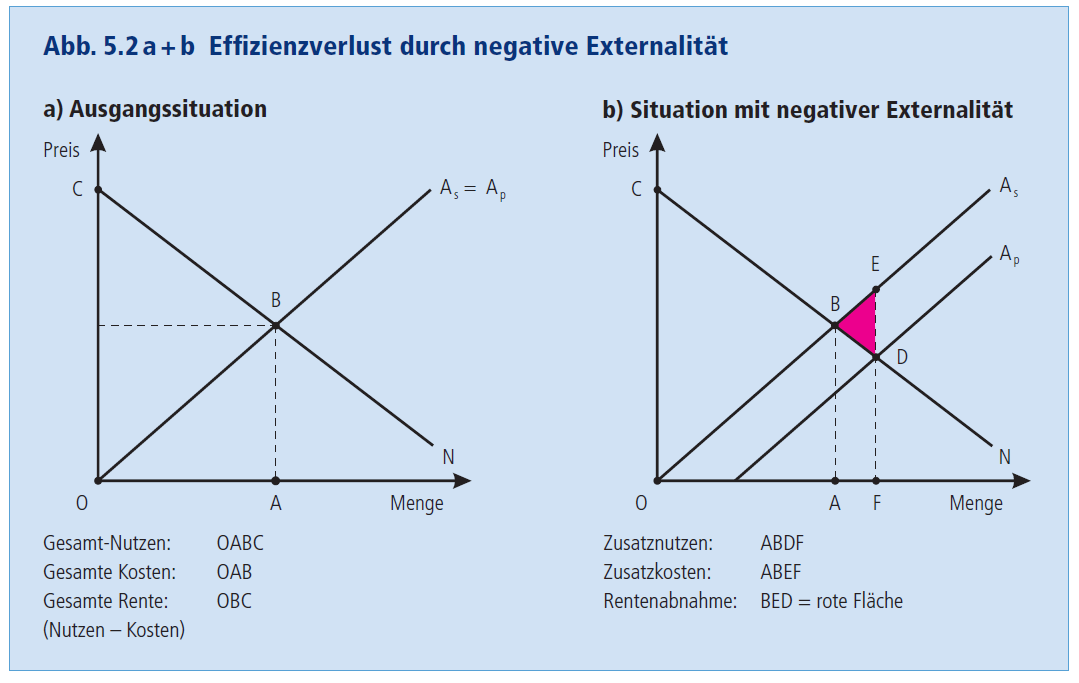
\includegraphics[width=9cm]{./bilder/h05f12.png}
	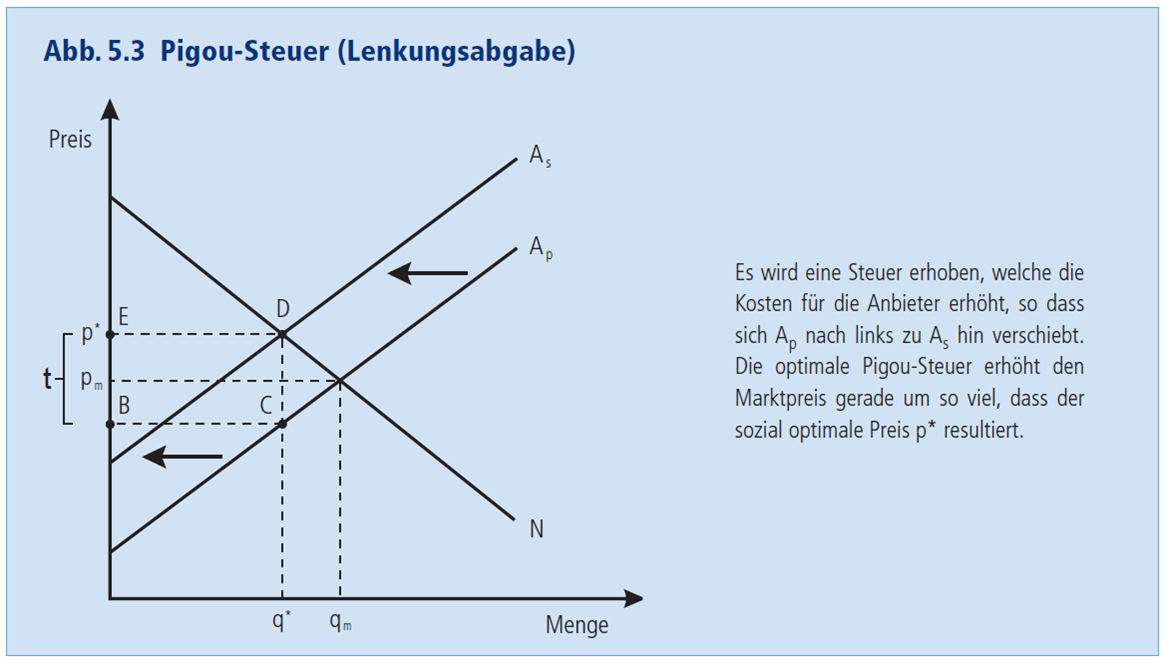
\includegraphics[width=9cm]{./bilder/h05f17.png}
\end{multicols}

\begin{multicols}{2}
\subsection{Langfristiges Wachstum \ho{Ho6}}
Konjunkturverlauf schwankt mehr als das langfristige Wachstum.
	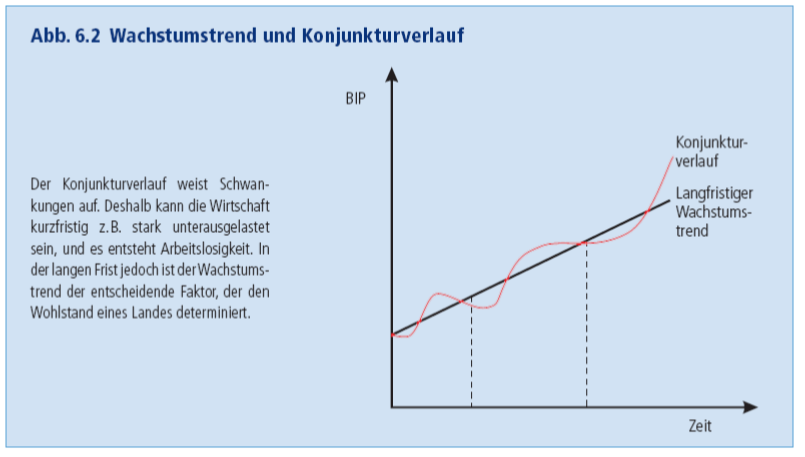
\includegraphics[width=9cm]{./bilder/h06f06.png}
\subsubsection{Technisches Know How \ho{Ho6 F7}}
  Technisches Know How ist der wichtigste Wachstumsfaktor, da er der Einzige ist
  der unbeschr�nkt verf�gbar ist.
  	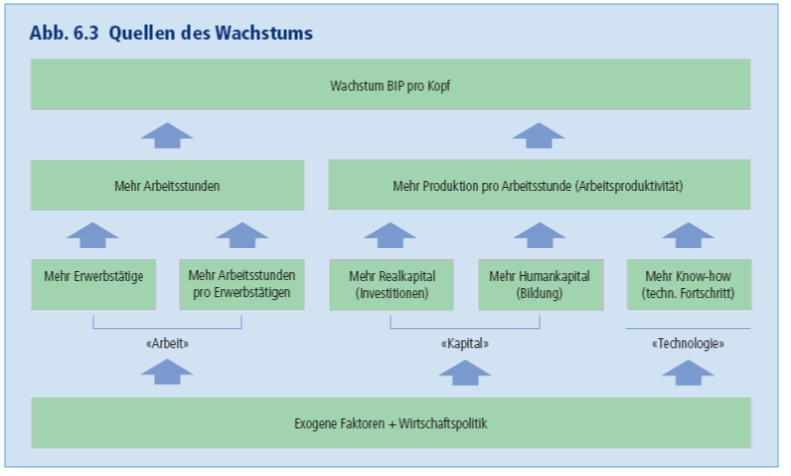
\includegraphics[width=9cm]{./bilder/h06f07.png}
 \end{multicols}
\subsubsection{Patentschutz \ho{Ho6 F11}}
  Patentschutz bietet einen Investitionsschutz, behindert aber technischen
  Fortschritt. Daher muss man dazwischen ein Mittel suchen. 
